%\documentclass[preprint,12pt]{elsarticle}
% \documentclass[preprint,review,12pt]{elsarticle}
%% \documentclass[final,1p,times]{elsarticle}
%% \documentclass[final,1p,times,twocolumn]{elsarticle}
%% \documentclass[final,3p,times]{elsarticle}
 \documentclass[final,3p,times,twocolumn]{elsarticle}
%% \documentclass[final,5p,times]{elsarticle}
%% \documentclass[final,5p,times,twocolumn]{elsarticle}

\usepackage{amssymb}
\usepackage{graphicx}
\usepackage{lineno}

\graphicspath{{../assets/}}

\journal{KIV/VI - Information Visualization}

\begin{document}

\begin{frontmatter}

\title{Does Showing Up Matter?\\
Lecture Attendance and Academic Outcomes\\
in a University Course}

\author[FAV]{Trong Quoc Huy Dinh}
\author[FAV]{Martin Reich\corref{corMR}}
\ead{trrolik511@gmail.com}
\author[FAV]{Eli\v{s}ka Toncarov\'{a}}

\cortext[corMR]{Corresponding author}

\address[FAV]{Department of Computer Science and Engineering,
Faculty of Applied Sciences, University of West Bohemia,
Plze\v{n}, Czech Republic}

\begin{abstract}
We present an interactive visualization dashboard that explores the
relationship between lecture attendance and academic performance across
15 years of student records from a university course at the University
of West Bohemia. The dataset covers 2\,740 evaluated students
(academic years 2010/11--2024/25), each tracked over 13 lecture weeks
per semester. Using a Plotly/Dash web application, we implemented seven
coordinated views -- including box plots, bar charts, scatter plots with
an OLS trendline, and a Sankey flow diagram -- backed by interactive
filters for year, class group, teaching day, exam-attempt number, and
attendance range. Our central finding is a steep pass-rate gradient:
students attending 0--3 weeks pass at only 55\,\%, while those
attending 10--13 weeks pass at 99\,\%. A moderate positive Pearson
correlation ($r \approx 0.39$) between attendance and final points
is confirmed across the full dataset. The COVID-19 remote-delivery
period (AY 2019/20--2020/21) affected only the lowest-attendance cohort,
whose pass rate fell by 17 percentage points, while higher-attendance
groups were unaffected.
\end{abstract}

\begin{keyword}
information visualization \sep attendance analysis \sep
academic performance \sep Plotly Dash \sep Sankey diagram
\end{keyword}

\end{frontmatter}

\linenumbers

%% ─────────────────────────────────────────────────────────────────────
\section{Introduction}

Student absenteeism is a persistent concern in higher education.
Lecturers, study advisors, and administrators routinely collect
attendance records, yet these data are rarely analysed in a systematic
and visually accessible way that would allow non-statistician
stakeholders to draw actionable conclusions.
The question of whether attendance actually predicts success -- or merely
correlates with latent motivation -- has been studied in the educational
psychology literature \cite{Credé2010}, but institution-level evidence
over a long time horizon is scarce.

This work addresses that gap for one mandatory computer-science course at
the University of West Bohemia.
The dataset spans 15 academic years (2010/11 -- 2024/25) and includes
per-week binary attendance flags, final grades (1--4, S, N), final
exam points, and the number of exam attempts for 2\,740 evaluated
students.
Our goal is twofold: (1) to surface the empirical relationships between
attendance and outcomes through a set of carefully chosen visualization
types, and (2) to provide an interactive tool that lets instructors and
study counsellors slice the data along dimensions that matter to them
(year, class group, teaching day, etc.).

The primary research questions are: Does attendance predict final grade
and exam points? Do low-attending students need more exam attempts to
pass? Is there an attendance threshold above which pass rates become
near-universal? What does the full attendance $\to$ attempts $\to$ grade
pathway look like in aggregate?


%% ─────────────────────────────────────────────────────────────────────
\section{Related Work}
\label{sec:relatedwork}

Meta-analyses of class attendance in tertiary education find consistent
positive correlations between attendance and grades \cite{Credé2010}.
Effect sizes vary across disciplines and institutions, but the
relationship is sufficiently robust to justify attendance-based
early-warning interventions.

On the visualization side, educational data mining commonly uses
bar charts and scatter plots to communicate grade distributions and
correlations \cite{Romero2010}.
Sankey diagrams have been applied to student-flow analyses, tracing
cohorts through enrolment, retention, and graduation stages
\cite{Aulck2017}.
Interactive dashboards built with web-based frameworks expose complex
multi-dimensional data to users who do not have a programming or
statistics background; Plotly Dash \cite{Plotly2015} is a widely used
Python framework for this purpose.
OLS regression trendlines embedded in scatter plots are a standard
technique for making linear associations visible without requiring the
reader to interpret a correlation coefficient \cite{Cleveland1985}.


%% ─────────────────────────────────────────────────────────────────────
\section{Methods}
\label{sec:methods}

\subsection{Data and preprocessing}

The dataset consists of one row per student per academic year with
the following columns: \texttt{academic\_year}, \texttt{class},
\texttt{day} (teaching day of the week), per-week binary attendance
flags \texttt{week\_1} through \texttt{week\_13},
\texttt{total\_attendance} (sum of attended weeks, 0--13),
\texttt{exam\_attempt} (integer, missing when no exam was taken),
\texttt{final\_grade} (1, 2, 3, 4, S, or N), and
\texttt{final\_points} (numeric, available for a subset of years).

Preprocessing is performed in pandas \cite{McKinney2010}:
weekly flags are summed to produce \texttt{total\_attendance};
students are classified into four attendance brackets
(0--3, 4--6, 7--9, 10--13 attended weeks);
and each student is assigned an outcome label
(\textit{Passed 1st attempt}, \textit{Passed (multiple attempts)},
or \textit{Did not pass}) based on whether any of their records
contain a passing grade (1, 2, 3, 4, or S) and on the minimum
exam-attempt number at which that grade was achieved.

\subsection{Visualization dashboard}

The application is built with Python, Plotly Express, and
Dash \cite{Plotly2015}.
It exposes seven view types selectable from a dropdown:

\begin{enumerate}
  \item \textbf{Attendance vs Final Grade} -- box, line, or scatter
        plot showing the distribution of attendance per grade category.
  \item \textbf{Attendance Distribution} -- box, line, or scatter plot
        showing how many students attended each number of lectures.
  \item \textbf{Exam Attempts vs Attendance} -- box, line, or scatter
        plot relating the number of exam attempts to total attendance.
  \item \textbf{Pass Rate by Attendance Bracket} -- grouped bar or line
        chart showing the fraction of students who passed, needed
        multiple attempts, or did not pass within each bracket.
  \item \textbf{Final Points vs Attendance} -- scatter plot with an
        OLS trendline; box and line variants also available.
  \item \textbf{Attendance vs Grade Flow (Sankey)} -- a Sankey diagram
        tracing students from attendance bracket through exam-attempt
        number to final grade.
  \item \textbf{Attendance by Teaching Day} -- box plot comparing
        attendance distributions across Monday--Friday cohorts.
\end{enumerate}

Each view can be further restricted by five interactive filters:
academic year, class group, teaching day, exam-attempt number, and
an attendance range slider (0--13).
Four KPI cards at the top of the dashboard always reflect the
currently visible cohort: student count, average attendance,
exam-participation rate, and the number of displayed rows out of
the total.

When a user switches view, the dashboard automatically snaps the
chart type and filter defaults to the most informative preset for
that view (e.g., the Sankey view defaults to the largest class group;
the Points vs Attendance view restricts to the most recent year and
students who have a recorded final-points value).

\subsection{OLS trendline}

For the scatter-plot view of final points vs attendance, a
custom OLS trendline is computed with \texttt{numpy.polyfit}
(degree 1) and rendered as a dashed black overlay.
The legend reports the fitted slope and $R^2$ so that the reader
can assess the strength of the linear relationship at a glance.


%% ─────────────────────────────────────────────────────────────────────
\section{Results}
\label{sec:results}

\subsection{Pass rate by attendance bracket}

The starkest finding is the step-wise increase in pass rate across
the four attendance brackets (Fig.~\ref{fig:passrate}).
Students attending 0--3 lectures pass at only 55\,\%, while the rate
rises to 91\,\% for 4--6 weeks, 95\,\% for 7--9 weeks, and
99\,\% for 10--13 weeks.
The jump between the lowest and the next bracket (+36 pp) is by far
the largest, suggesting that crossing the threshold of attending
roughly one-third of lectures is the single most important behavioural
factor for passing.

\begin{figure}[h]
  \centering
  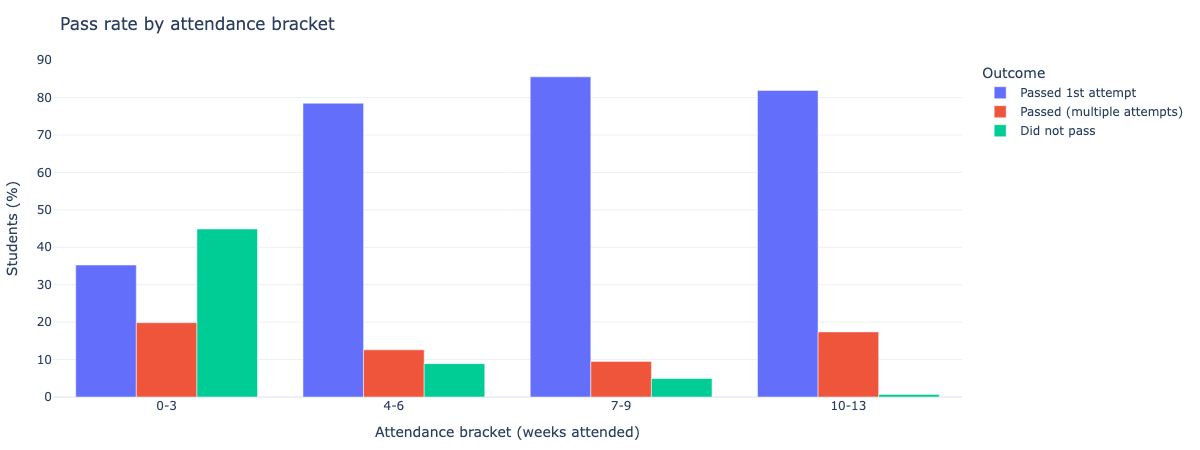
\includegraphics[width=\linewidth]{fig_passrate.png}
  \caption{Pass rate by attendance bracket. The grouped bar chart
           separates \textit{Passed 1st attempt},
           \textit{Passed (multiple attempts)}, and
           \textit{Did not pass} for each of the four brackets.}
  \label{fig:passrate}
\end{figure}

\subsection{Attendance and final points}

The scatter plot with OLS trendline (Fig.~\ref{fig:points}) shows a
moderate positive linear relationship between total attendance
(0--13 weeks) and final exam points.
The Pearson correlation across the full dataset is $r \approx 0.39$.
The fitted slope indicates that each additional attended lecture is
associated with roughly 1.5--2 additional points on the final exam.
Substantial scatter around the trendline confirms that attendance is
a contributing factor, not a deterministic one: a sizeable minority
of high-attenders score low, and some low-attenders score high.

\begin{figure}[h]
  \centering
  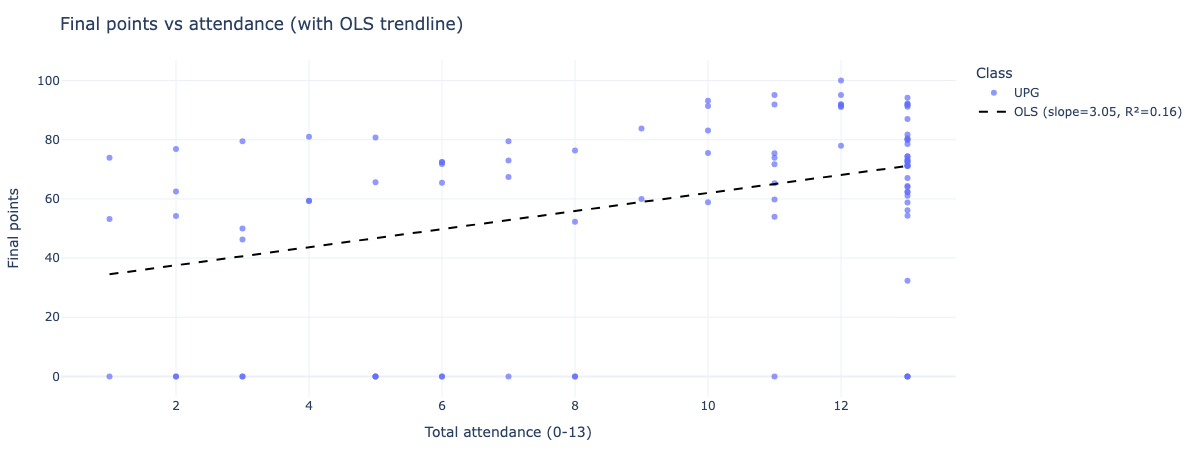
\includegraphics[width=\linewidth]{fig_points.png}
  \caption{Scatter plot of final points vs total attendance with
           OLS trendline ($r \approx 0.39$).
           Each point represents one student; colour encodes
           class group.}
  \label{fig:points}
\end{figure}

\subsection{Attendance and final grade}

The box plot in Fig.~\ref{fig:grade} shows the distribution of
attendance for each final grade category.
Students who received the best grade (1) attended on average more
than 3 additional lectures compared with students who failed (N or S).
The medians decrease monotonically from grade 1 to N, and the
inter-quartile ranges overlap substantially, again consistent with
a moderate rather than deterministic relationship.

\begin{figure}[h]
  \centering
  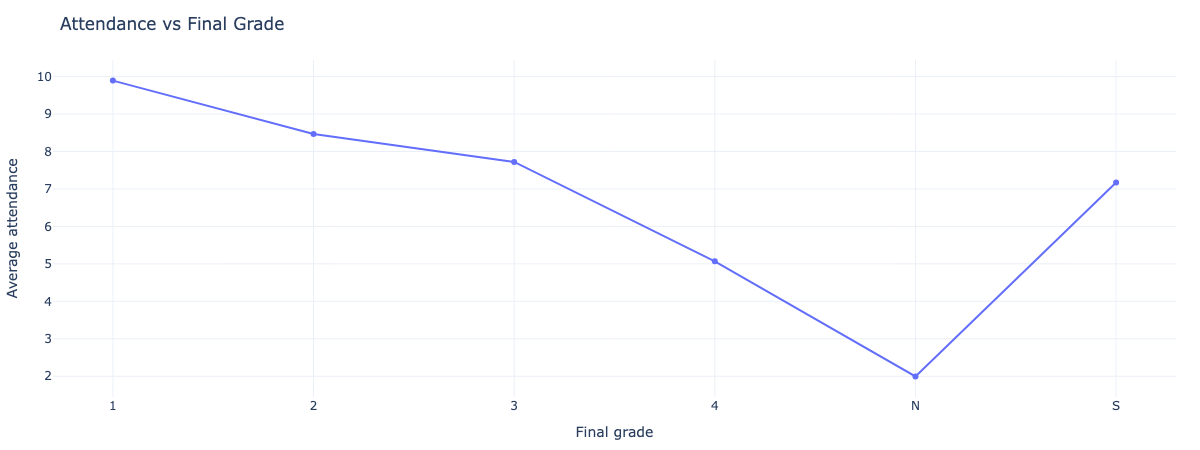
\includegraphics[width=\linewidth]{fig_grade.png}
  \caption{Attendance distribution per final grade.
           Grade 1 is the best outcome; N indicates failure.}
  \label{fig:grade}
\end{figure}

\subsection{Exam attempts and attendance}

Fig.~\ref{fig:attempts} shows that students who needed more exam
attempts had, on average, lower attendance.
First-attempt passers cluster near the upper end of the attendance
range, whereas repeat-attempt students show a notably lower median
and more low-attendance outliers.

\subsection{Sankey flow diagram}

The Sankey diagram (Fig.~\ref{fig:sankey}) traces the complete
pathway from attendance bracket through exam-attempt number to
final grade.
It makes visually apparent that the failure stream -- students
ending up with grade N -- is almost entirely fed by the 0--3 bracket,
while the 10--13 bracket overwhelmingly flows into first-attempt
grade-1 or grade-2 outcomes.
The diagram also reveals that a non-trivial flow from the 4--6
bracket requires two or three attempts before passing.

\begin{figure}[h]
  \centering
  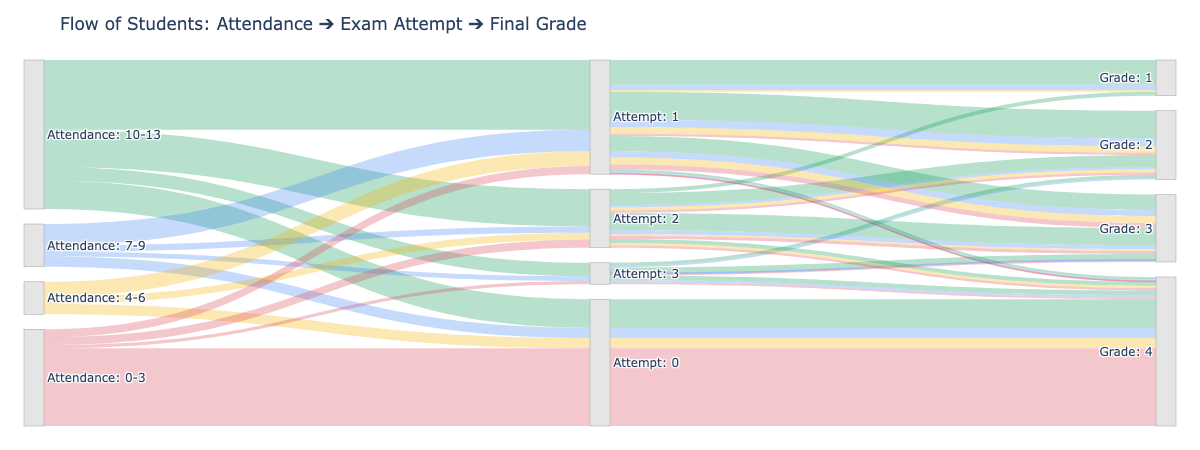
\includegraphics[width=\linewidth]{fig_sankey.png}
  \caption{Sankey diagram: attendance bracket $\to$
           exam-attempt number $\to$ final grade.
           Link colour is inherited from the source attendance bracket.}
  \label{fig:sankey}
\end{figure}

\subsection{COVID-19 remote-delivery period}

Restricting the data to AY 2019/20 and 2020/21 (352 students,
average attendance 6.09/13) reveals that the pandemic affected
outcomes asymmetrically.
Low-attenders (0--3 weeks) saw their pass rate fall from 55\,\% to
38\,\% (-17 pp).
Medium-attenders (4--9 weeks) were stable or marginally improved
($\approx$93\,\% $\to$ $\approx$96\,\%).
High-attenders (10--13 weeks) were virtually unaffected
(99\,\% $\to$ 98\,\%).
This finding suggests that online delivery disproportionately
hurt students who were already the most disengaged.


%% ─────────────────────────────────────────────────────────────────────
\section{Discussion}
\label{sec:discussion}

The positive association between attendance and performance is
stable across 15 academic years and robust to the COVID disruption
at moderate and high attendance levels.
However, the moderate correlation ($r \approx 0.39$) means that
attendance explains roughly 15\,\% of the variance in final points.
The remaining 85\,\% is driven by factors outside this dataset:
prior knowledge, study habits, ability, and motivation.

The most important caveat is \textbf{self-selection bias}.
Students who are motivated and well-prepared tend both to attend
more often and to perform better.
The association we observe is therefore not necessarily causal.
A randomised experiment assigning compulsory vs optional attendance
would be needed to isolate the causal effect.

A second limitation is that the dataset covers a single course
at a single institution, which limits generalisability.
The attendance-performance gradient might be weaker in courses
with different pedagogical structures (e.g., fully recorded lectures
or problem-based learning).

Third, students who withdrew from the course or never registered
for the exam are excluded from the pass-rate calculations, which
may slightly inflate the apparent pass rate for low-attendance students
(those students may have been even worse performers who are not
counted as failures).

Despite these limitations, the dashboard is practically useful.
The steep pass-rate jump at the 4-week threshold provides a clear,
actionable boundary for early-warning systems: students absent in
the first three weeks of the semester can be flagged for outreach
before the midterm, while there is still time to improve attendance.


%% ─────────────────────────────────────────────────────────────────────
\section{Future Work}
\label{sec:futurework}

Several extensions would deepen the analysis.
First, examining per-week attendance curves (weeks 1--13 individually)
could reveal whether early-semester absence is a stronger predictor
than late-semester absence, enabling finer-grained intervention timing.

Second, integrating a simple logistic-regression or
gradient-boosting classifier into the dashboard would allow
instructors to obtain, after the first few weeks, a probability
estimate for each student of eventually passing the course.

Third, expanding the dataset to multiple courses across the faculty
would enable cross-subject comparisons and test whether the
attendance--performance gradient generalises beyond a single course.

Fourth, adding anonymised prior-achievement data (e.g., high-school
leaving-exam scores) would make it possible to partial out the
self-selection effect via regression adjustment or propensity-score
matching, yielding a cleaner causal estimate.

Finally, the dashboard could be extended with a real-time data-import
pipeline so that lecturers can monitor the current semester's
attendance in the same tool, rather than relying on retrospective
analysis.


\section*{Acknowledgement}
The authors thank the staff of the Department of Computer Science
and Engineering at the University of West Bohemia for providing
access to the anonymised attendance records.

\bibliographystyle{elsarticle-num-names}
\bibliography{BibTexReferences}

\end{document}